\documentclass[12pt]{article}

\usepackage[english]{babel}
\usepackage[utf8]{inputenc}
\usepackage{fancyhdr}

\usepackage[margin=1in]{geometry}
\usepackage{pgf}
\usepackage{pgfplots}
\usepackage{siunitx}
\usepackage{tikz}
\usepackage{float}
\usepackage{amsmath}
\usepackage{enumitem}

\usepackage[font=small,labelfont=bf]{caption}
\usepackage{pstricks-add}
\usepackage{pgfplotstable}
\usepackage[nodisplayskipstretch]{setspace}

\usetikzlibrary{scopes}
\usetikzlibrary{angles,quotes}
\usetikzlibrary{calc}
\pgfplotsset{compat=1.5}
\graphicspath{ {/} }

\newcommand*{\I}{\imath}
\newcommand*{\J}{\jmath}
\newcommand{\norm}[1]{\lvert #1 \rvert}

\setlist[enumerate, 1]{label=\alph*.}

\begin{document}
\sisetup{per-mode=symbol}

\begin{titlepage}
    \begin{center}
        \vspace*{1cm}
        \textbf{Electric Circuits}

        \vspace{0.5cm}
        Lab: 01

        \vspace{1cm}

        \textbf{Jaden Moore}

        \vfill

        Orange Coast College\\
        Engineering Circuits A285\\
        November 17th, 2021

    \end{center}
\end{titlepage}

\pagestyle{fancy}
\fancyhf{}
\setlength{\headheight}{15pt}
\lhead{Electric Circuits}
\rhead{Lab: 01}
\cfoot{\thepage}

\section{Introduction}
In this lab, we utilize standard DC circuit theory to analyze the voltages and currents at various nodes and elements  within three different circuits and then compare our analysis to computer-aided design (CAD) circuit software to obtain a percent error between the two. In this case, we are utilizing the online circuit simulator CircuitLab\textregistered\space to compare with our theoretical circuit analysis.

\section{Circuit 1}

\begin{figure}[H]
    \begin{center}
        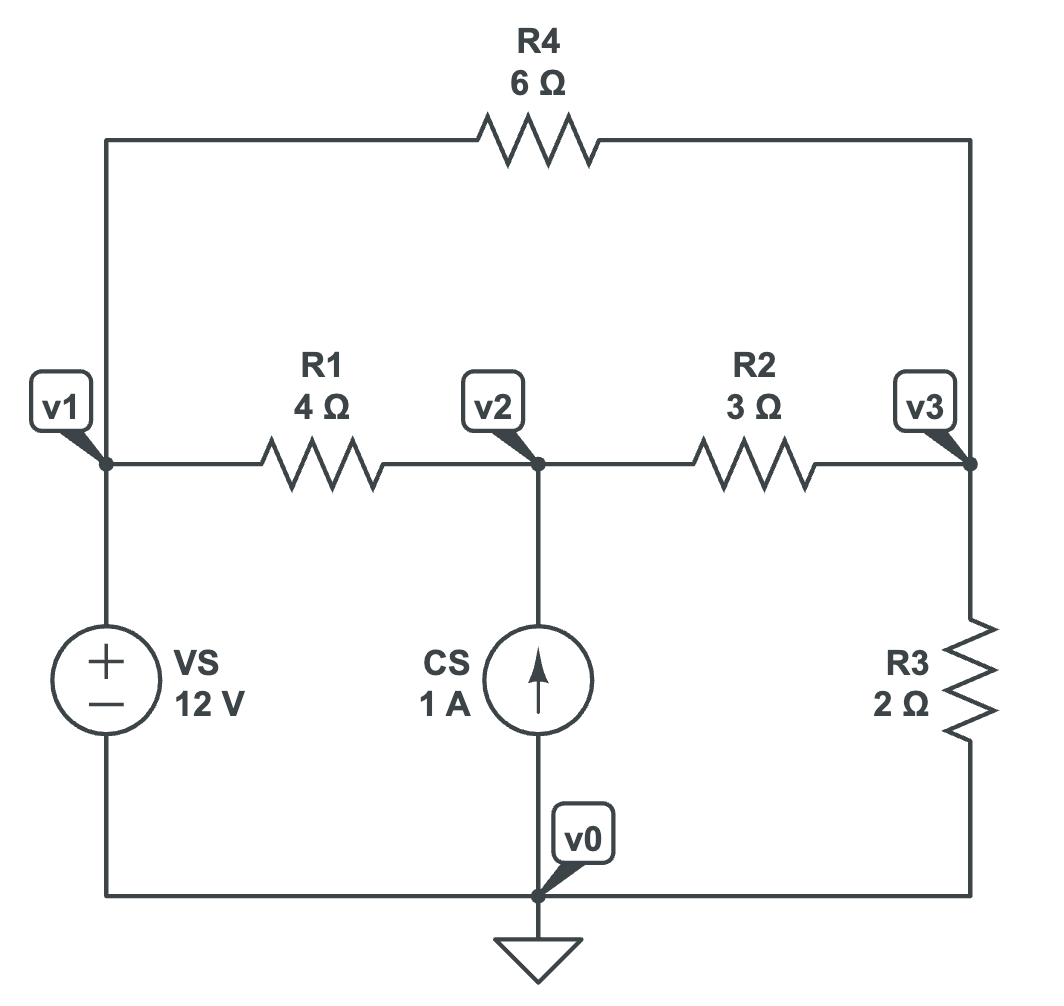
\includegraphics[scale=0.6]{circuit-1.png}
        \caption { Circuit 1}
    \end{center}
\end{figure}

Consider the voltages at the specified nodes in Figure (1). We can apply nodal analysis to determine the voltages at each node and then utilize CircuitLab to simulate the circuit and confirm our results.

\subsection{Circuit 1 Analysis}

(a) Following the path $ v_0 \rightarrow v_s \rightarrow v_1$, we see that 

\begin{equation}
    \begin{split}
        v_1 = \SI{12}{\volt}
    \end{split}
\end{equation}

Applying Kirchhoff's current law (KCL) to $v_2$, we get the node equation

\begin{equation}
    \begin{split}
        \frac{v_2 - 12}{4} + \frac{v_2 - v_3}{3} - 1 = 0 \implies 7v_2 - 4v_3 = 48
    \end{split}
\end{equation}

Applying KCL to node $v_3$ we get

\begin{equation}
    \begin{split}
         \frac{v_3 - v_2}{3} + \frac{v_3 - 12}{6} + \frac{v_3}{2} = 0 \implies -4v_2 + 12v_3 = 24
    \end{split}
\end{equation}

Solving Equation (2) for $v_3$ and putting it into Equation (1) we get that

\begin{equation}
    \begin{split}
         7v_2 - 4\left(\frac{24+4v_2}{12}\right) = 48 \implies v_2 = \SI{9.882}{\volt}
    \end{split}
\end{equation}

Putting $v_2$ back into Equation (2) we get $v_3$ to be

\begin{equation}
    \begin{split}
        -4(9.882) + 12v_3 = 24 \implies v_3 = \SI{5.294}{\volt}
    \end{split}
\end{equation}

(b) Using the node voltages, We can calculate the current through any branch using Ohm's Law. That is,

\begin{equation*}
    \begin{split}
        i = \frac{\Delta v}{R}
    \end{split}
\end{equation*}

Thus, from theory, the current through each resistor can be calculated such that

\begin{equation}
    \begin{split}
        i_1 &= \frac{v_1 - v_2}{R_1} = \frac{12 - 9.882}{4} = \SI{529.4}{\milli\ampere} \\
        i_2 &= \frac{v_2 - v_3}{R_2} = \frac{9.882 - 5.294}{3} = \SI{1.529}{\ampere} \\
        i_3 &= \frac{v_3 - v_0}{R_3} = \frac{5.294 - 0}{2} = \SI{2.647}{\ampere} \\
        i_4 &= \frac{v_1 - v_3}{R_4} = \frac{12 - 5.294}{6} = \SI{1.118}{\ampere}
    \end{split}
\end{equation}

\subsection{Circuit 1 Results}
\begin{figure}[H]
    \begin{center}
        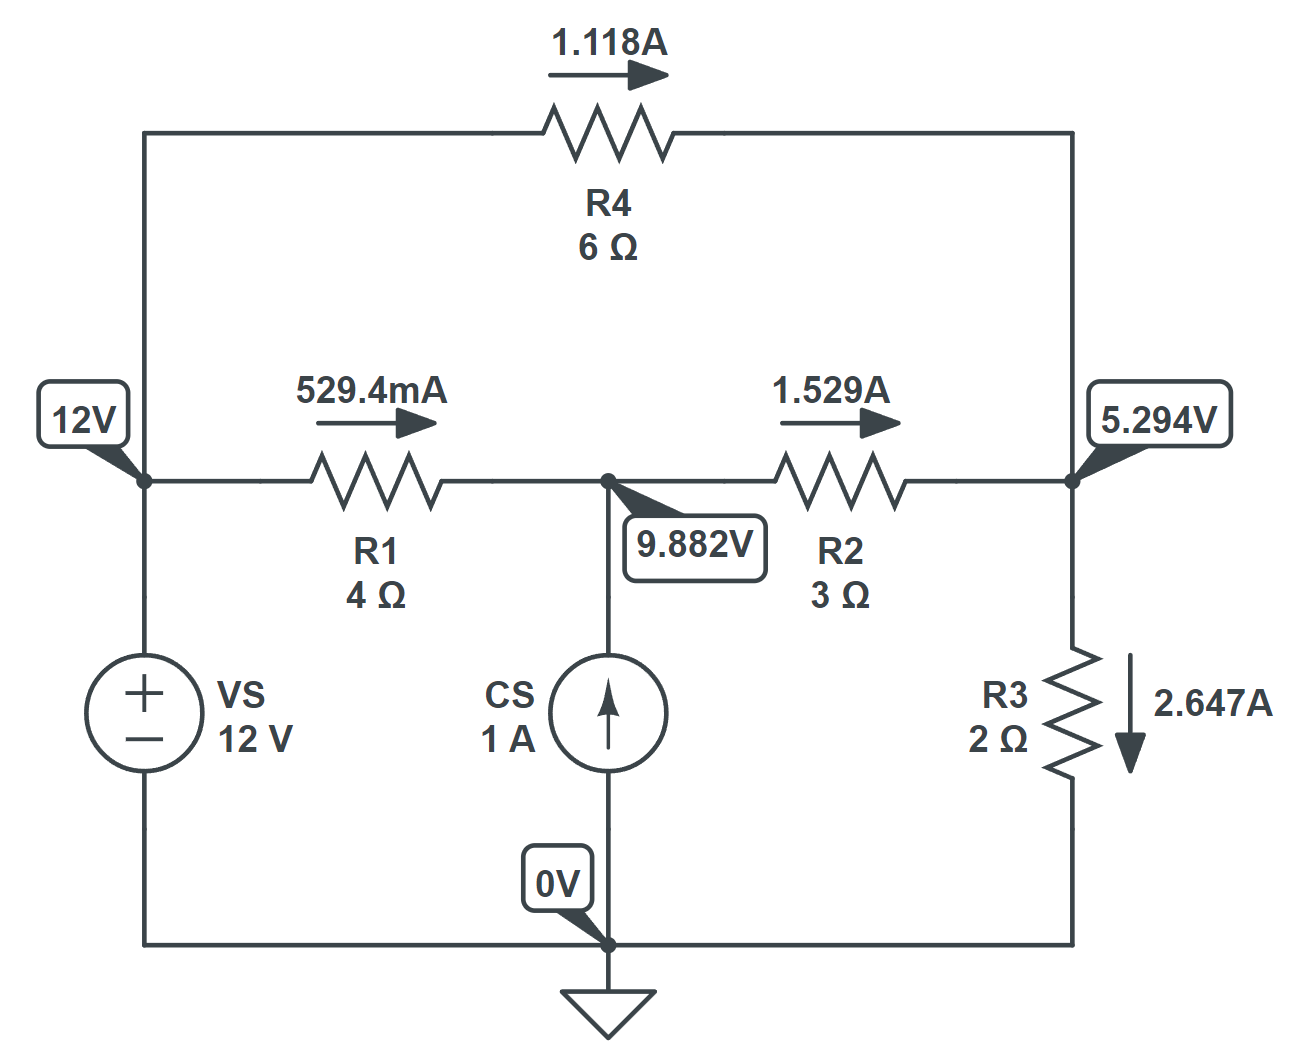
\includegraphics[scale=0.6]{circuit-1-sol.png}
        \caption { Circuit 1 CAD Simulation Results}
    \end{center}
\end{figure}

In this case, we see that the CAD simulation produced the same currents through each resistor as calculated by theory which confirms our method was accurate with a 0\% error between the two. The simulation produced equivalent node voltages and currents with respect to the theoretical values.

\section{Circuit 2}
\begin{figure}[H]
    \begin{center}
        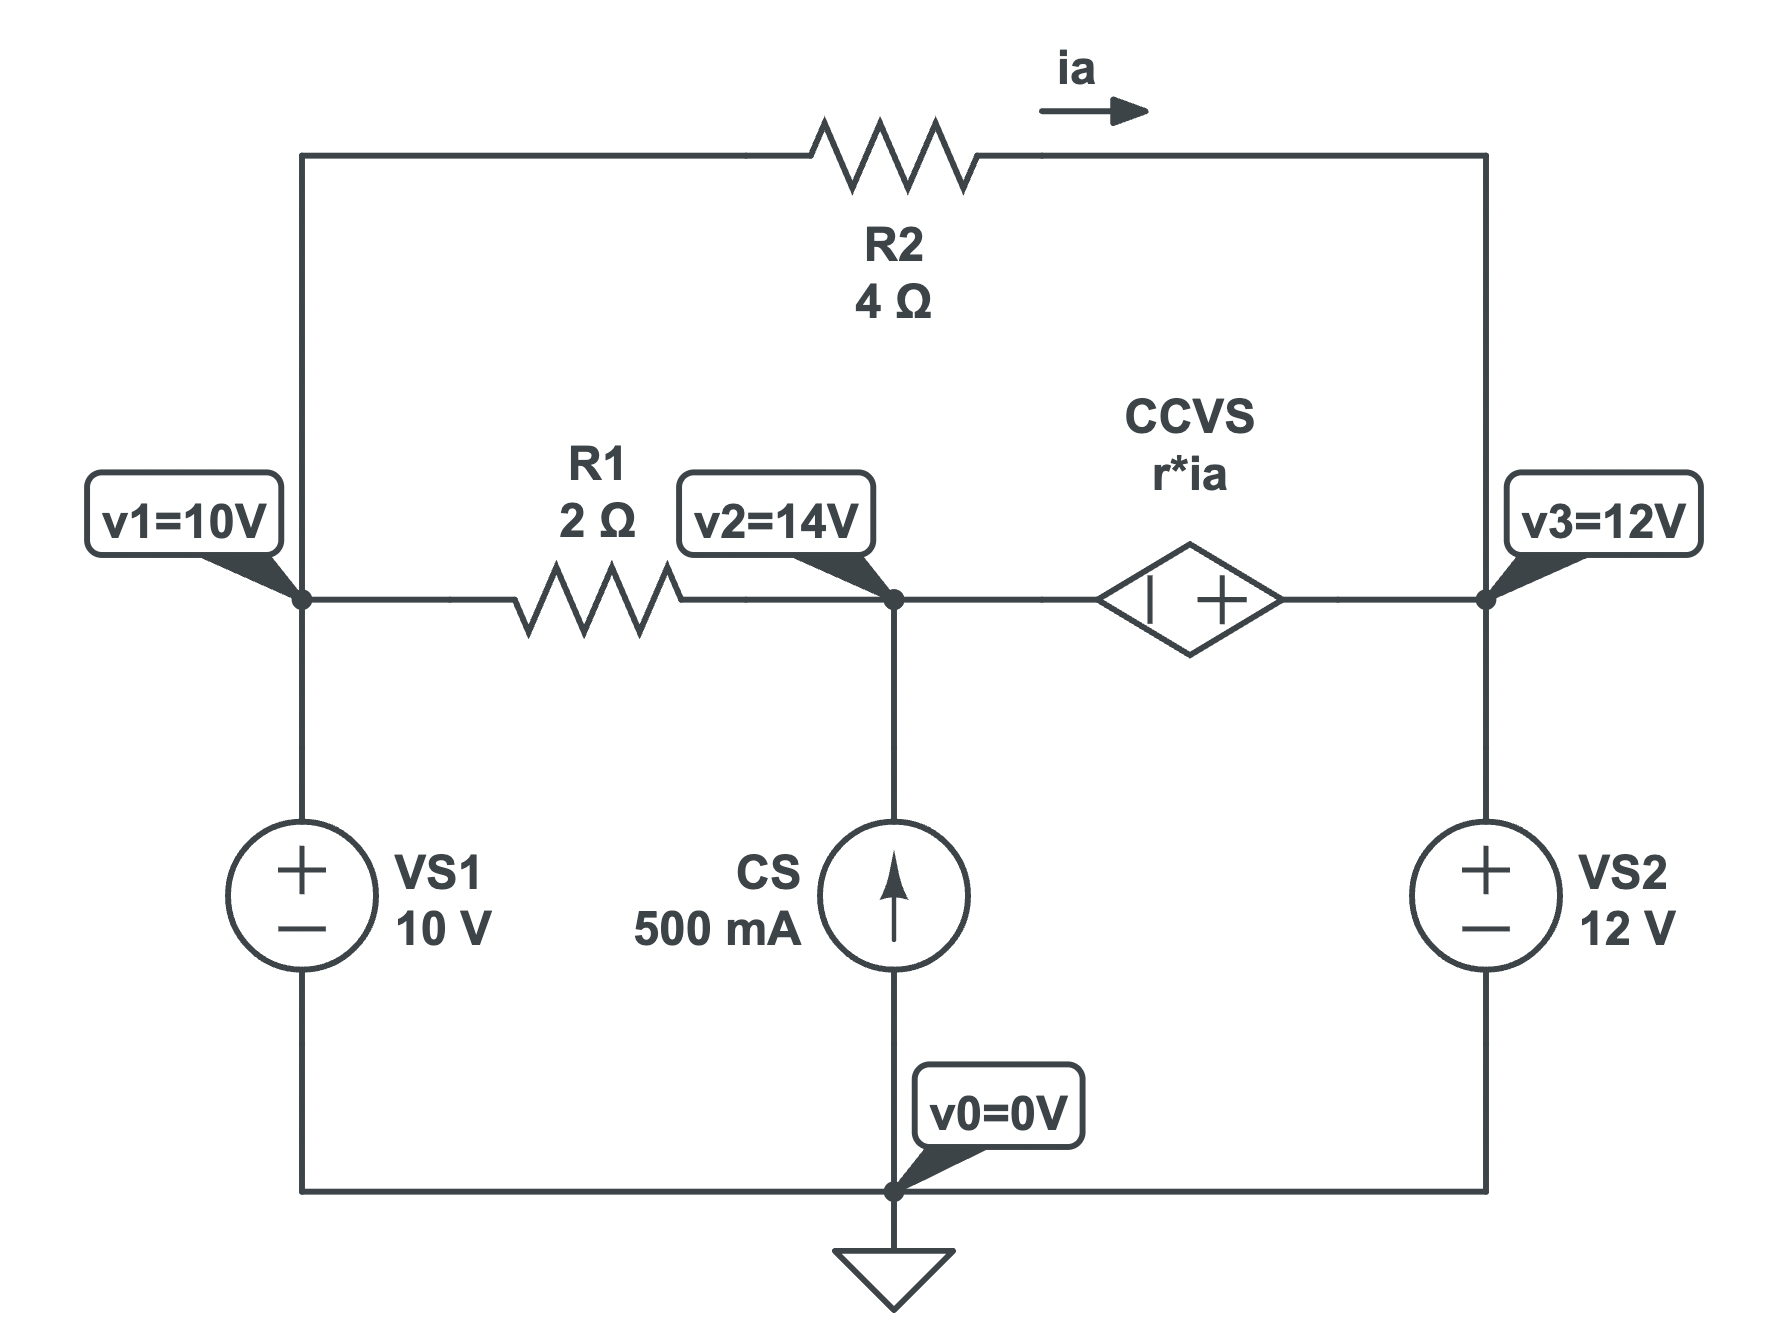
\includegraphics[scale=0.5]{circuit-2.png}
        \caption { (a) Circuit 2}
    \end{center}
\end{figure}


Consider the gain $r$ of the current controlled voltage source (CCVS) in Figure (3). 

\subsection{Circuit 2 Analysis}
(b) We can calculate the gain of the source by considering the values of the voltage at nodes $v_2$ and $v_3$. That is, we can express the relationship between the CCVS its adjacent nodes such that

\begin{equation}
    \begin{split}
        ri_a = v_3 - v_2
    \end{split}
\end{equation}

But $i_a$ can be expressed by

\begin{equation}
    \begin{split}
        i_a = \frac{v_1-v_3}{R_2} = \frac{10 - 12}{4} = \SI{-0.5}{\ampere}
    \end{split}
\end{equation}

Thus, substituting back into Equation (7), we get

\begin{equation}
    \begin{split}
        r(-0.5) = 12 - 14 \implies r = \SI{4}{V/A}
    \end{split}
\end{equation}

(c) If instead we let $v_2 = \SI{16}{V}$, we can quickly calculate the gain of the CCVS such that

\begin{equation}
    \begin{split}
        r(-0.5) = 12 - 16 \implies r = \SI{8}{V/A}
    \end{split}
\end{equation}

Thus, $r = \SI{8}{V/A}$ when $v_2 = \SI{16}{V}$

\subsection{Circuit 2 Results}

In this case, from part c, we realize that we can calculate the gain of the CCVS no matter what the voltages are at its adjacent nodes. Furthermore, the results gathered from the CircuitLab simulation of Figure (3) are consistent with the results obtained in section 3. That is, there is a 0\% error between the theory and the CAD simulation. Giving a value of $r=\SI{4}{V/A}$ gives the correct node voltages in the simulation.

\section{Circuit 3}

\begin{figure}[H]
    \begin{center}
        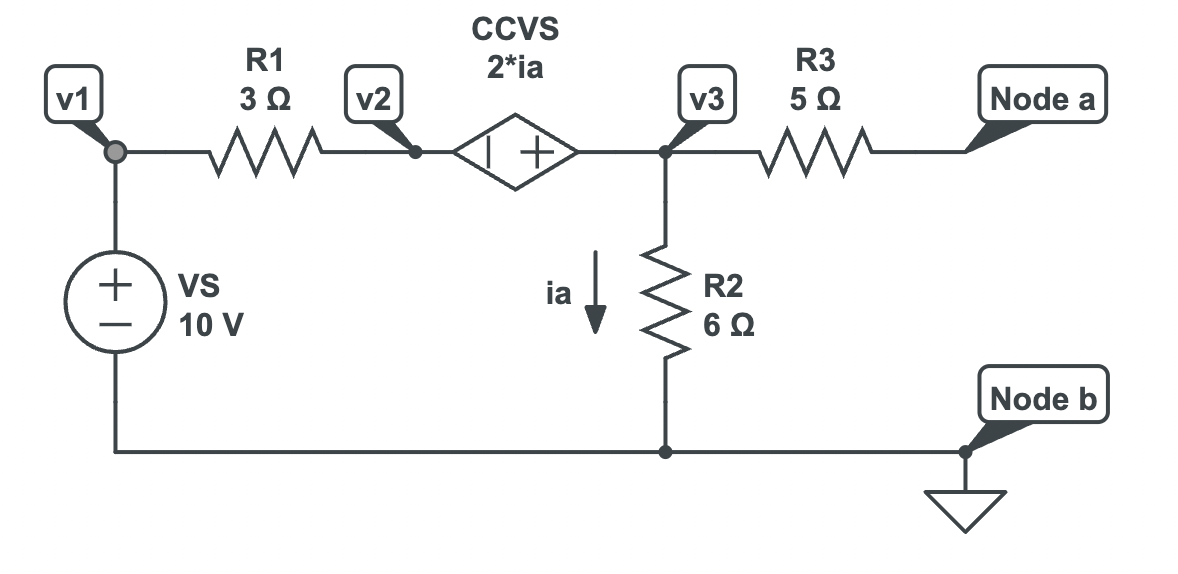
\includegraphics[scale=0.5]{circuit-3.png}
        \caption { (a) Circuit 3}
    \end{center}
\end{figure}

\end{document}